\section{Mod\`ele \`a un seul pool de MO}
\subsection{Description du mod\`ele}

\begin{equation}
  {{d[BC]}\over{dt}} =
  \left ( Y_{BC} u_{BC} - kd_{BC} \right ) [BC]
  \label{eq:eq1}
\end{equation}
\begin{equation}
  {{d[TOC]}\over{dt}} =
  -ec [BC]
  \label{eq:eq2}
\end{equation}
\begin{equation}
  {{d[SBC]}\over{dt}} =
  ec [BC] - u_{BC} [BC]
  \label{eq:eq3}
\end{equation}
\begin{equation}
  {{d[SNH_4]}\over{dt}} =
  vNH_4 - nitri
  \label{eq:eq4}
\end{equation}

\par{
Avec
}

\begin{equation}
  ec = e_{1mx} {{[TOC]}\over{k_{1h} + [TOC]}}
  \label{eq:eq5}
\end{equation}
\begin{equation}
  vNH_4 = u_{BC} [BC] (NC)_{TOC} - Y_{BC} u_{BC} [BC] (NC)_{BC}
  \label{eq:eq6}
\end{equation}
\begin{equation}
  nitri = nimax {{[NH_4]}\over{k_{NH_4ni}+[NH_4]}}
  \label{eq:eq7}
\end{equation}

\subsection{Simulation de r\'ef\'erence}

\begin{figure}[h!]
  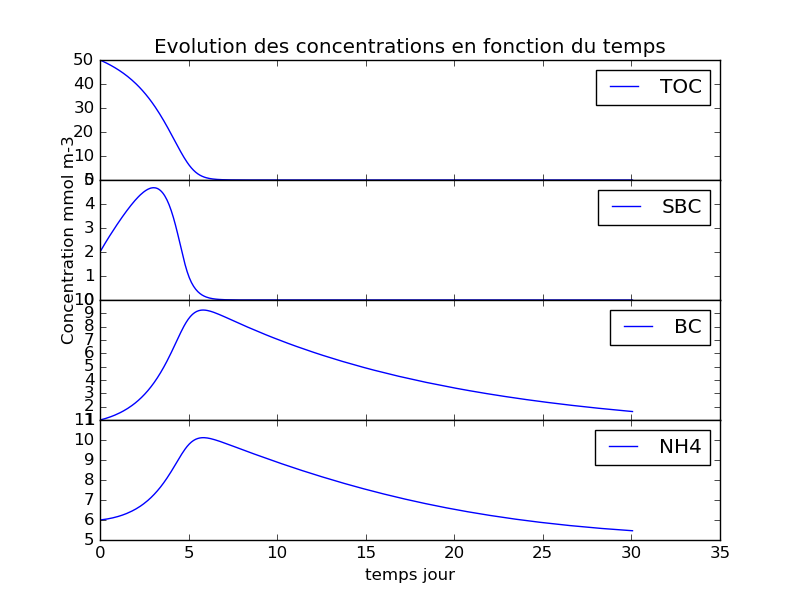
\includegraphics[width=\textwidth]{partie1/Ref.png}
  \caption{Simulation de r\'ef\'erence, pour un mod\`ele \`a un seul pool de mati\`ere organique
  }
  \label{fig:partie1ref}
\end{figure}

\subsection{Test 1}

\begin{figure}[h!]
  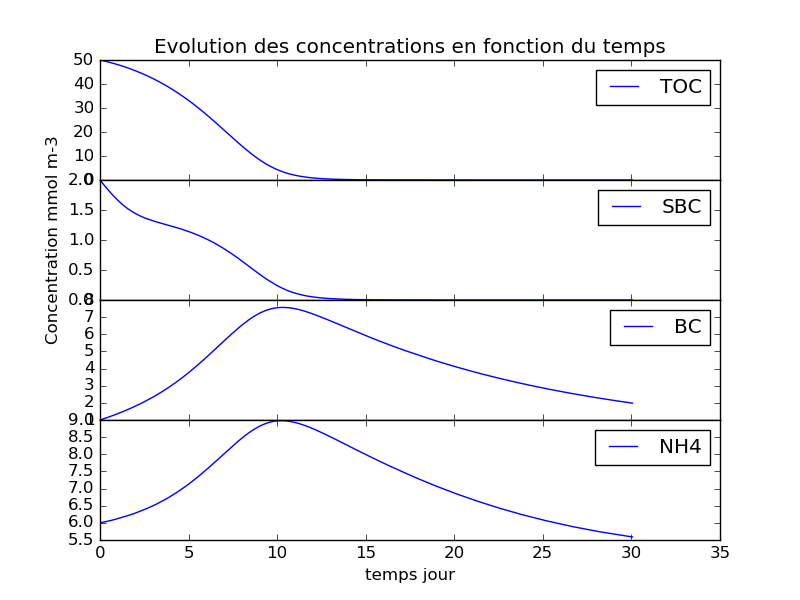
\includegraphics[width=\textwidth]{partie1/Test1.png}
  \caption{Simulation de r\'ef\'erence, pour un mod\`ele \`a plusieurs pools de mati\`ere organique
  }
  \label{fig:partie1test1}
\end{figure}

\subsection{Test 2}

\begin{figure}[h!]
  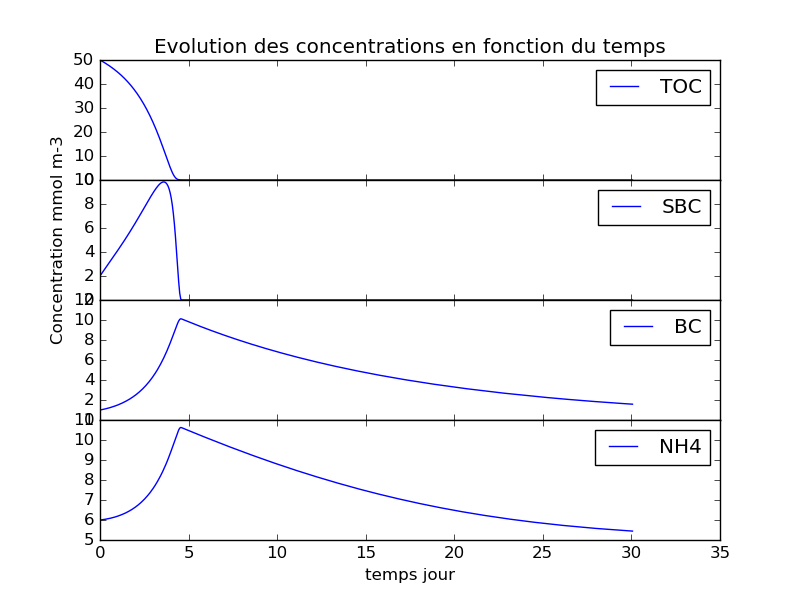
\includegraphics[width=\textwidth]{partie1/Test2.png}
  \caption{Simulation de r\'ef\'erence, pour un mod\`ele \`a plusieurs pools de mati\`ere organique
  }
  \label{fig:partie1test2}
\end{figure}

\subsection{Test 3}

\begin{figure}[h!]
  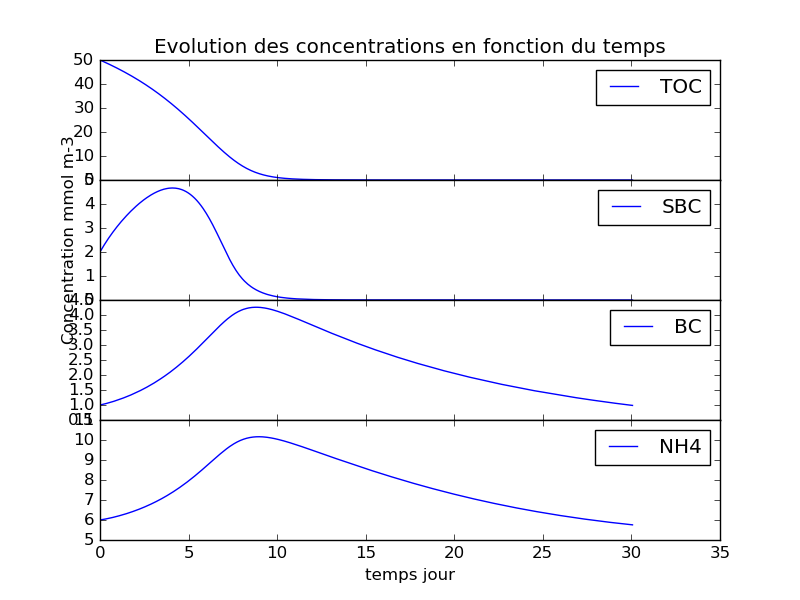
\includegraphics[width=\textwidth]{partie1/Test3.png}
  \caption{Simulation de r\'ef\'erence, pour un mod\`ele \`a plusieurs pools de mati\`ere organique
  }
  \label{fig:partie1test3}
\end{figure}

\subsection{Test 4}

\begin{figure}[h!]
  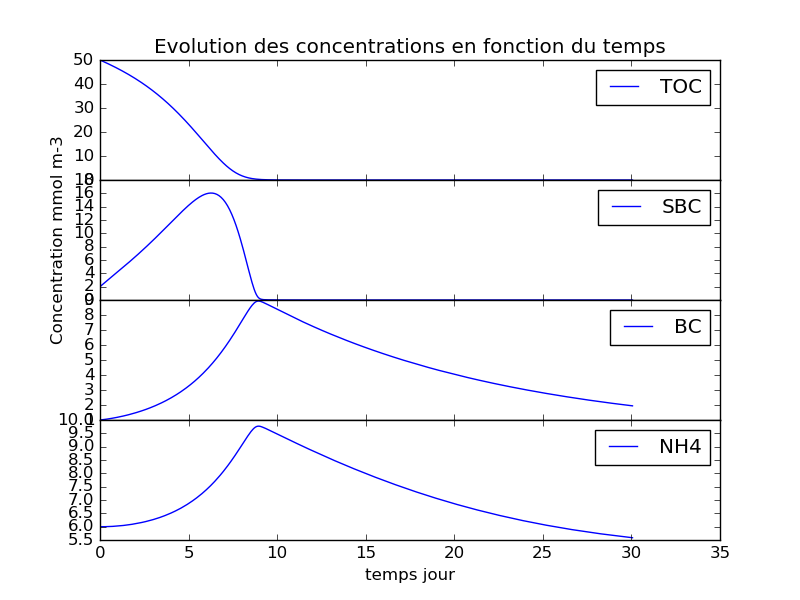
\includegraphics[width=\textwidth]{partie1/Test4.png}
  \caption{Simulation de r\'ef\'erence, pour un mod\`ele \`a plusieurs pools de mati\`ere organique
  }
  \label{fig:partie1test4}
\end{figure}

\subsection{Test 5}


\begin{figure}[h!]
  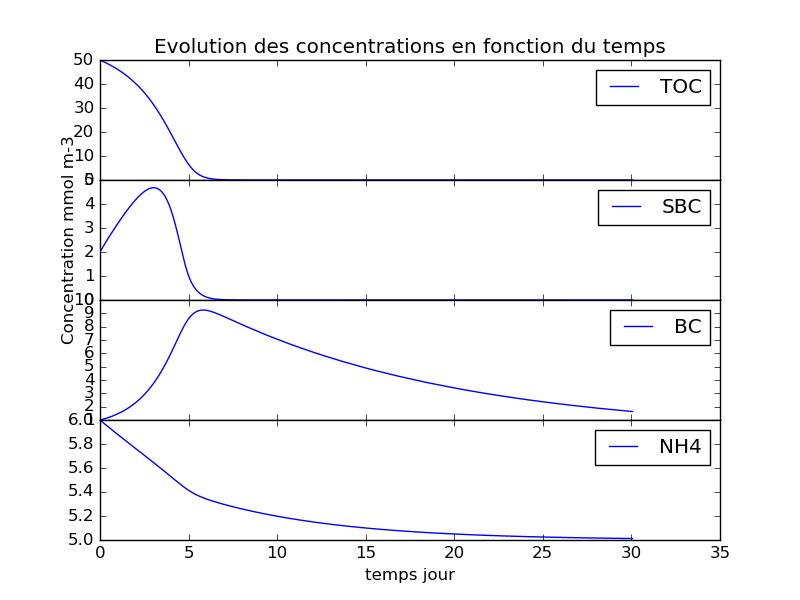
\includegraphics[width=\textwidth]{partie1/Test5.png}
  \caption{Simulation de r\'ef\'erence, pour un mod\`ele \`a plusieurs pools de mati\`ere organique
  }
  \label{fig:partie1test5}
\end{figure}

